\documentclass[11pt]{article}
\usepackage[round]{natbib}
\usepackage{amsmath}
\usepackage{graphicx}
\usepackage[margin=1in]{geometry}
\usepackage[colorlinks,citecolor=blue]{hyperref}

\title{Minimum Wages and Teen Employment: Evidence from County Borders}
\author{Daniel Reyes\thanks{Department of Economics, University of Arizona. Email:
\texttt{dreyes@example.edu}.} \and Grace Liu}
\date{Working paper, August 2026}

\begin{document}
\maketitle

\begin{abstract}
We compare contiguous county pairs that straddle state borders to estimate the effect of
minimum wage increases on teen employment. Our estimates suggest an employment
elasticity close to zero, in line with recent border-discontinuity studies.
\end{abstract}

\section{Introduction}
The employment effect of minimum wages is one of the most studied questions in labour
economics. Early time-series work found substantial disemployment effects
\citep{brown1982}, whereas the case study of \citet{card1994} found none.
Subsequent work has used ever finer comparisons \citep[see][for a review]{neumark2008};
\citet{dube2010} pioneered the contiguous county-pair design that we extend here.

\section{Empirical strategy}
For county $c$ in pair $p$ at time $t$ we estimate
\begin{equation}
\ln E_{cpt} = \alpha + \eta \ln MW_{ct} + \beta X_{ct} + \phi_c + \tau_{pt} + \varepsilon_{cpt},
\label{eq:main}
\end{equation}
where $\tau_{pt}$ are pair-by-period fixed effects. The coefficient $\eta$ is identified
from differences within each pair, as argued by \citet[p.~950]{dube2010}.

\section{Results}
Figure~\ref{fig:event} plots event-study coefficients. The estimate of $\eta$ in
\eqref{eq:main} is $-0.04$ (s.e.\ $0.06$), and we cannot reject zero
\citep{card1994,dube2010}.

\begin{figure}[t]
\centering
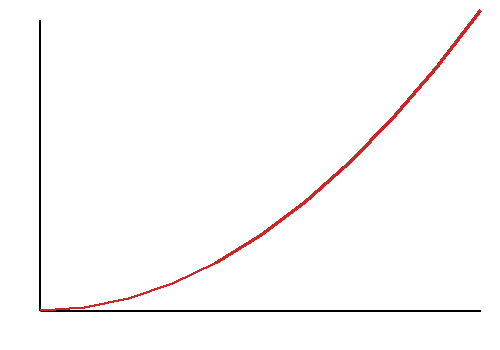
\includegraphics[width=0.75\linewidth]{plot.png}
\caption{Event-study estimates with 95\% confidence intervals.}
\label{fig:event}
\end{figure}

\section{Conclusion}
Our results are consistent with monopsony models of the low-wage labour market
\citep{manning2003}.

\bibliographystyle{plainnat}
\begin{thebibliography}{5}
\providecommand{\natexlab}[1]{#1}
\bibitem[Brown et~al.(1982)Brown, Gilroy, and Kohen]{brown1982}
Charles Brown, Curtis Gilroy, and Andrew Kohen.
\newblock The effect of the minimum wage on employment and unemployment.
\newblock \emph{Journal of Economic Literature}, 20\penalty0 (2):\penalty0 487--528, 1982.

\bibitem[Card and Krueger(1994)]{card1994}
David Card and Alan~B. Krueger.
\newblock Minimum wages and employment: A case study of the fast-food industry in New
  Jersey and Pennsylvania.
\newblock \emph{American Economic Review}, 84\penalty0 (4):\penalty0 772--793, 1994.

\bibitem[Dube et~al.(2010)Dube, Lester, and Reich]{dube2010}
Arindrajit Dube, T.~William Lester, and Michael Reich.
\newblock Minimum wage effects across state borders.
\newblock \emph{Review of Economics and Statistics}, 92\penalty0 (4):\penalty0 945--964, 2010.

\bibitem[Manning(2003)]{manning2003}
Alan Manning.
\newblock \emph{Monopsony in Motion}.
\newblock Princeton University Press, 2003.

\bibitem[Neumark and Wascher(2008)]{neumark2008}
David Neumark and William Wascher.
\newblock \emph{Minimum Wages}.
\newblock MIT Press, 2008.
\end{thebibliography}

\end{document}
